\documentclass{article}
\usepackage{graphicx}
\usepackage{hyperref}

\begin{document}

\title{The HypeDyn Hypertext Fiction Editor\\Tutorial 2: Alternate Links,
Conditional Text and Anywhere Nodes}
% \author{Alex Mitchell}
\date{}

\onecolumn
\maketitle

\tableofcontents


\section{Introduction}
In this tutorial, we will introduce some new features to HypeDyn:

\begin{itemize}
  \item ``alternate links'', which can be followed when a rule on a link is
  \textit{not} satisfied;
  \item ``conditional text'', which can be displayed \textit{instead of} the
  original text in a link when a rule on a link is not satisfied; and
  \item ``anywhere nodes'', which are nodes that don't form part of the main
  hypertext, but are automatically added as links at the bottom of all regular
  nodes.
\end{itemize}

In this tutorial, we will be creating a variation of the ``Little Red
Riding Hood'' hypertext fiction which you created in tutorial 1. We will change
the story such that the reader is able to choose whether Red is naive or
street-smart, which will have consequences as to how the story ends. We will
also add a ``summary'' node, reachable from all other nodes, which show an
up-to-date summary of the story so far.

% \textit{Note: For users of Ariadne, you will find most of the functionality of
% HypeDyn familiar. You may, however, want to quickly run through tutorial 1, as
% this tutorial assumes that you have a HypeDyn version of the original Little
% Red Riding Hood story.}

\begin{figure}[h]
  \centering
  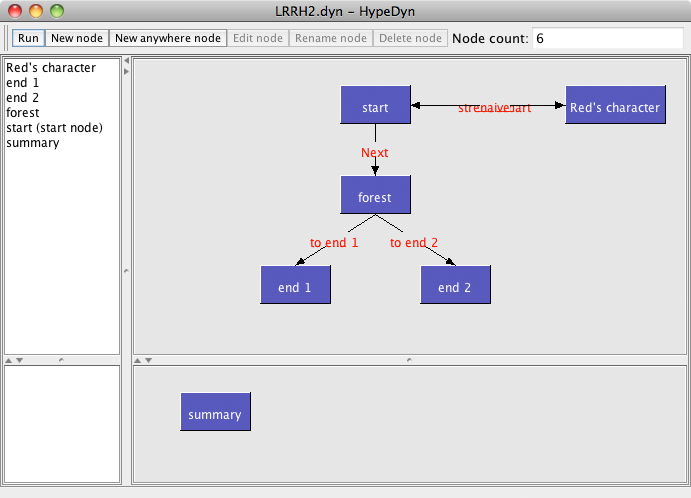
\includegraphics[width=10cm]{images/hypedyn-tutorial-2-figure-1}
  \caption{\textit{The completed ``Little Red Riding Hood'' story.}}
\end{figure} 

The nodes and links in the final story are shown in Figure 1.

\textit{Note:  HypeDyn is a work-in-progress, so there are some features that are still
not completed, and there may be bugs. If you encounter any errors, please
report them as bugs on our Launchpad site: \url{https://launchpad.net/hypedyn}.}

\section{Getting started}

First, open HypeDyn by double-clicking on the file \textbf{HypeDyn.exe} (in
Windows) or \textbf{HypeDyn.app} (in MacOS).

We will continue from the story that you created in tutorial 1. If you don't
have the story, you can start from the file \textsc{LRRH.dyn} in the
\textsc{examples} folder. HypeDyn files always end with a \textbf{.dyn} extension.

% \textit{Note: for users of Ariadne, the HypeDyn file format is different
% from the Ariadne file format. If you have your LRRH.xml file from the Ariadne tutorial,
% you will not be able to load it in HypeDyn.}

We no longer need the ``Hood details'' node, so delete this node by clicking on
the node in either the node list on the left of the main window, or in the
map view on the right of the main window, and then clicking the ``Delete node''
button. Save the resulting file under a different name.

\section{Creating an alternate link}

The first new feature we will introduce is the ``alternate link''. This feature
allows you to specify a second destination for a link, which will only be
followed if the rule in the link is \textit{not} satisfied.

For our story, we want to provide two different endings: one ending if Red is
naive, and a second ending if she is street-smart. We will provide one link for
the reader to click on and, depending on the choice that the reader made at the
start of the story, the link will lead to either the first or the second ending.

\subsection{Letting the reader make a choice}

To let the reader make a choice, we will create a node named ``Red's
character'', which contains two links, one to a node named ``Red is naive'' and
another to a node named ``Red is street-smart''. We will then create a
condition on the ``to the end'' link in the ``forest'' node which leads
to node ``end1'' if node ``Red is naive'' was visited, and otherwise goes to
node ``end2''.

\begin{enumerate}
  \item Create a new node named ``Red's character''. In the new node, enter the
following text:

\begin{quotation}
Is Red naive or street-smart?
\end{quotation}

\item Next, create a new node named ``Red is naive''. In the new node, enter the
following text:

\begin{quotation}
Red is naive.

back
\end{quotation}

\item Make a link from the text ``back'' to the ``start'' node (see Figure 2).
Notice that the \textit{Edit link} dialogue contains a list of conditions
(initially empty), plus a \textit{THEN} and an \textit{ELSE} section. The
actions listed in the \textit{THEN} section will be performed if the rule
defined by the conditions is satisfied, otherwise the actions in the
\textit{ELSE} section will be performed. For our link, we just want to specify
that the link should be followed to the ``start'' node, with no conditions, so
just check the checkbox under the \textit{THEN} section, and choose the
``start'' node in the list to the right of ``follow link to''.

\begin{figure}[h]
  \centering
  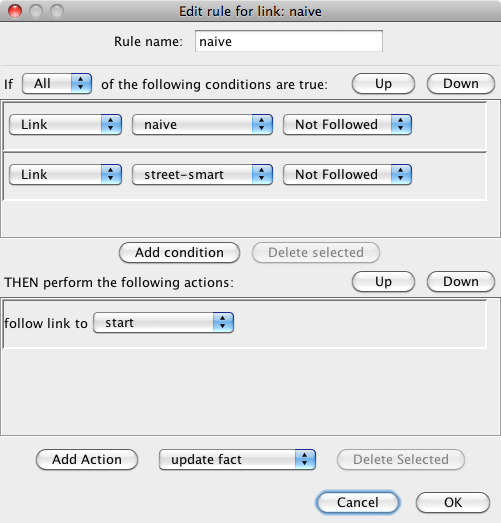
\includegraphics[width=9cm]{images/hypedyn-tutorial-2-figure-2}
  \caption{\textit{A regular link from ``Red is naive'' to ``start''.}}
\end{figure} 

\item Now create a new node named ``Red is street-smart''. In the new node,
enter the following text:

\begin{quotation}
Red is street-smart.

back
\end{quotation}

\item As with the ``Red is naive'' node, make a link from the text ``back'' to
the ``start'' node.
\item Next, edit the ``Red's character'' node by selecting it in the map
view and clicking the ``Edit node'' buton. Make a link from the text ``naive''
to the node ``Red is naive''. Since we don't want the reader to be able to
change their choice, we will put a condition on this link: the link can only be
followed if the reader \textit{hasn't} visited both the nodes ``Red is naive''
and ``Red is street-smart'' (see Figure 3).

\begin{figure}[h]
  \centering
  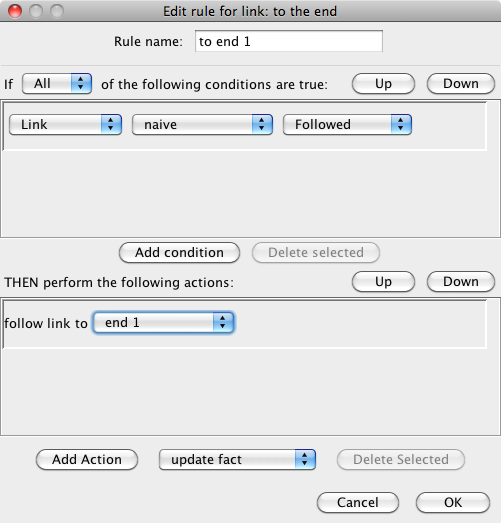
\includegraphics[width=9cm]{images/hypedyn-tutorial-2-figure-3}
  \caption{\textit{Adding conditions on the link to ``Red is naive''.}}
\end{figure} 

\item Do the same to create a link from the text ``street-smart'' in the node
``Red's character'' to the node ``Red is street-smart''.
\item Finally, edit the node ``start'', and make a link from the text ``Little
Red Riding Hood'' to the node ``Red's character'', with condition ``Red's
Character'' is not visited. This will prevent the reader from being able to go
in and make their choice a second time.

Note that even though we put this condition on the link to ``Red's character'',
we still need the conditions on the links from ``Red's character'' to the two
nodes representing her character, just in case the reader presses the ``back''
button and tries to change their choice.
\end{enumerate}

Now we have the mechanism in place to let the reader choose what sort of person
Red is: naive or street-smart. We can now check which of the two nodes were
visited, ``Red is naive'' or ``Red is street-smart'', whenever we want to make
a decision which is influenced by Red's character. This is an example of using
the visited state of a node as a way of representing some information about the
state of the storyworld. This is a very useful technique which can be
generalized to allow for more complex, dynamic behaviour.

\subsection{Following a link based on the reader's choice}

Now we will create the link to the two different endings, and follow the link
to the appropriate ending based on the reader's choice about Red's character.

\begin{enumerate}
  \item First, rename the current ``end'' node to ``end 1'' by selecting the
  node in the map view, and clicking on the ``Rename node'' button. Type in the
  new name, and click ``Ok''.
  \item Edit the node ``end 1'', and delete the text ``back to start''. Notice
  that the link to the ``start'' node is deleted when you delete the text.
  \item Next, replace the text in the node ``end 1'' with the following text:
  \begin{quotation}
  Quickly the wolf ran ahead to Grandma's house, swallowed Grandma whole, and
  disguised himself as the poor old lady. When Red arrived, he finished her
  off too. Yum!

  *** The End ***
  \end{quotation}
  \item Now create a new node, named ``end 2'', and enter the following text:
  \begin{quotation}
  Frustrated, the wolf snuck off to try his luck at the mall instead.

  *** The End ***
  \end{quotation}
\end{enumerate}

Now that we have the two endings in place, we need to make sure that the link
from the text ``next'' in node ``forest'' takes the reader to ``end 1'' if Red
is naive. Otherwise (ie. if Red is street-smart), the link should take the
reader to ``end 2''. To do this, we will use the \textit{ELSE} action in the
\textit{Edit link} dialogue.

\begin{enumerate}
  \item Edit the ``to the end'' link on the text ``next'' in node ``forest''.
  The original link, from the previous version of the story, has an
  unconditional link to the original end node, now renamed ``end 1'' (see
  Figure 4).
\begin{figure}[h]
  \centering
  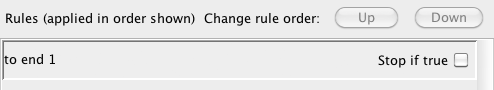
\includegraphics[width=9cm]{images/hypedyn-tutorial-2-figure-4}
  \caption{\textit{Original link from the ``forest'' node.}}
\end{figure} 
  Add two conditions: that the link should be followed if node ``Red is
  naive'' \textit{was} visited, and if node ``Red is street-smart'' was
  \textit{not} visited. Make sure that the list to the right of the ``IF'' at
  the top of the \textit{Edit link} dialogue box shows the ``All'' option -
  this means that \textit{all} of the conditions must be satisfied.
\end{enumerate}
This gives us the required behaviour for a naive Red. However, if the
conditions are \textit{not} satisfied, ie. if Red is street-smart, the link
won't go anywhere. Next we need to use the same link, but now specify what
should happen in this case.

\begin{enumerate}
  \item Still editing the link ``to the end'' in the node ``forest'', check the
  checkbox to the left of ``follow the link to'' in the \textit{ELSE} section,
  and choose the node ``end 2'' (see Figure 5).
\begin{figure}[h]
  \centering
  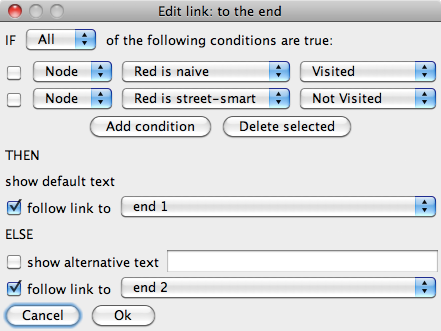
\includegraphics[width=9cm]{images/hypedyn-tutorial-2-figure-5}
  \caption{\textit{Specifying an alternative destination for a link.}}
\end{figure} 
\end{enumerate}

This alternative destination will be followed if the conditions listed are
\textit{not} satisfied.

\subsection{Forcing the reader to make a choice}

At this point we seem to have everything in place for the reader to make a
choice which impacts the end of the story. However, with our current
implementation, if the reader ignores the link on the text ``Little Red Riding
Hood'' in the ``start'' node, and goes through to the end of the story, she will
always end up with the second ending, since the conditions on the link we just
created will never be satisfied.

To fix this, we need to force the reader to make the choice about Red's
character \textit{before} we let her move on to the ``forest'' node. We can do
this by putting a condition on the link from ``start'' to ``forest'' such that
the link can only be followed if \textit{either} node ``Red is naive''
\textit{or} node ``Red is street-smart'' have been visited.

\begin{enumerate}
  \item Edit the link ``next'' in node ``start''.
  \item Add the condition ``Red is naive'' was visited
  \item Add the condition ``Red is street-smart'' was visited
  \item Change the list to the right of ``IF'' to show ``Any'' (see Figure 6).
\end{enumerate}

\begin{figure}[h]
  \centering
  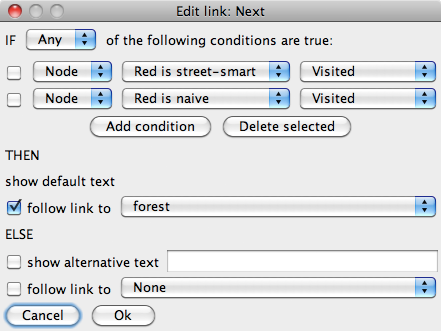
\includegraphics[width=9cm]{images/hypedyn-tutorial-2-figure-6}
  \caption{\textit{Specifying two conditions where \textbf{either} can be
  satisfied.}}
\end{figure} 

This means that the link will be followed if \textit{any} of the listed
conditions are satisfied, which is what we want.

\subsection{Testing the story}

Now that we have our story in place, we can test the story. You can do this by
clicking the ``Run'' button. The ``Run'' button will read the story starting at
the node which was set as the \textit{start} node, which will be indicated by the
text ``(start)'' to the right of the node name in the node list.

Try clicking through the story. You should be able to choose Red's character, and
then see a different ending based on your choice. You can stop reading by either
closing the ``Reader'' window, or by clicking the ``Stop'' button.

\section{Specifying conditional text}

As you read through the story, you probably realized that there's a problem:
the story doesn't really make sense. There's no explanation as to why the wolf
was unable to eat Red if she's street-smart. It also doesn't seem reasonable
that, as a street-smart little girl, she would have told the wolf that she was
going to Grandma's house.

So, it would be good if we could change what Red says to the wolf depending on
what choice the reader made regarding Red's character. This is where
\textit{conditional text} is useful.

What we want to do is set a condition so that, if the reader has chosen for
Red to be street-smart, the text ``I'm off to see my sick granny'' in the
``forest'' node will automatically be changed to ``I'm not supposed to talk to
strangers.''

\begin{enumerate}
  \item Edit the node ``forest''.
  \item Select the text ``I'm off to see my sick granny'', and click on
  ``New link''.
  \item In the ``New link" dialogue, name the link ``response'', and click
  ``ok''. You should see the ``Edit link'' dialogue.
  \item In the ``Edit link'' dialogue, add a condition, and set the condition
  to ``Red is street-smart'' is \textit{not} visited. This means that the
  link's \textit{THEN} actions will be performed if Red is naive, and its
  \textit{ELSE} actions will be performed if Red is street-smart.
  \item Since we don't want the reader to actually be able to click on this
  link, leave the \textit{THEN} destination's checkbox unchecked. This means
  that, if the conditions are satisfied, the default text will be shown, and
  nothing else will happen. The link will not be underlined or bold.
  \item If the conditions are \textit{not} satisfied, we still don't want the
  reader to be able to be able to click, but we \textit{do} want something to
  happen - we want the text to change. Do this by checking the checkbox to the
  left of ``show alternative text'' under the \textit{ELSE} section, and enter
  the text (see Figure 7):
  \begin{quotation}
  ``I'm not supposed to talk to strangers.''
  \end{quotation}
  \item Click on ``ok'' to close the ``Edit link'' dialogue. Note that the node
  as displayed in the map view is now shown as a ``stack'' of nodes - this is
  to remind you that you've created conditional text on this node.
\end{enumerate}

\begin{figure}[h]
  \centering
  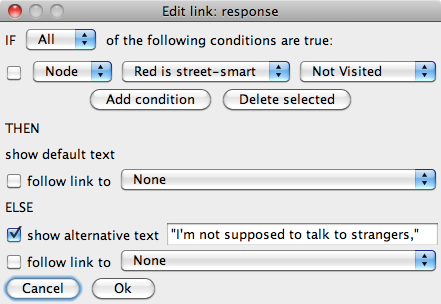
\includegraphics[width=9cm]{images/hypedyn-tutorial-2-figure-7}
  \caption{\textit{Specifying alternative text.}}
\end{figure} 

That's it! Now test the story by clicking on the ``Run'' button. You should see
the appropriate text in the ``forest'' node, depending on which personality you
chose for Red.

This is a simple feature, but it is a major addition to what can be done in
HypeDyn. Text is no longer fixed - the author can procedurally alter/generate
text within a node, based on the reader's actions.

\section{Anywhere nodes}

The last thing we are going to do is to add in an ``anywhere'' node. This is a
node which is automatically linked from all the nodes in the story. This
feature is useful as a way to create, for example, a summary of the story so
far, or a list of the decisions that the reader has made. 

\subsection{Adding the anywhere node}
In our case, we will create a summary of the story so far using an anywhere
node.

\begin{enumerate}
  \item Click on ``New anywhere node'', and name the new node ``summary''.
  Notice that the new node appears in the lower half of the map view - this is
  where ``anywhere'' nodes, which aren't part of the main hypertext, will
  appear.
  \item Edit the node by selecting it and clicking on ``Edit node'', as with a
  regular node.
  \item In the node, enter the following text:
  \begin{quotation}
  Red's character has been decided.
  She told the wolf where she is going.
  The end.
  \end{quotation}
\end{enumerate}

\subsection{Adding some conditional text}
We want the first line to be displayed after the reader has decided on Red's
character, the second line after the ``forest'' node has been visited, and the
third line once the reader has reached the end of the story. We can do this
using conditional text, as shown in the previous section.

\begin{enumerate}
  \item Select the first line of text, and click on ``New link''. Name the link
  ``character'' and click ``ok''.
  \item You should now see the ``Edit link'' dialogue (see Figure 8). Notice
  that it is a bit different from the regular ``Edit link'' dialogue - the \textit{THEN} and
  \textit{ELSE} sections no longer show a destination node. This is because you
  cannot make links from ``anywhere'' nodes to nodes in the hypertext.
\begin{figure}[h]
  \centering
  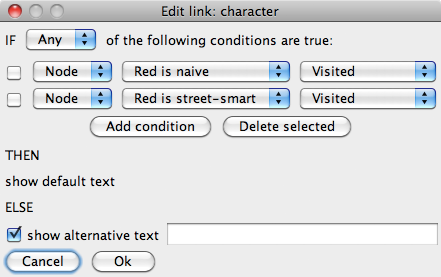
\includegraphics[width=9cm]{images/hypedyn-tutorial-2-figure-8}
  \caption{\textit{Editing a link on an anywhere node.}}
\end{figure} 
\item Now we want to set the conditions for when this text appears. Since we
want the first line to show after the reader has chosen Red's character, we
need two conditions: the node ``Red is naive'' has been visited, \textit{or}
the node ``Red is street-smart'' has been visited. Add these two conditions.
\item Since we want the text to show when either of these nodes has been
visited, set the type of the rule to ``Any''.
\item Finally, if the conditions are \textit{not} met, we want to show nothing,
so check the checkbox beside ``show alternative text'' in the \textit{ELSE}
section, and leave the text blank.
\item Click ``Ok'' to close the ``Edit link'' dialogue.
\end{enumerate}

\subsection{Adding the remaining conditional text}
Now do the same for the second and third lines:

\begin{enumerate}
  \item Add a link, named ``forest'', on the second line.
  \item Add one condition, that the ``forest'' node has been visited.
  \item Check the ``show alternative text'' checkbox, and leave the text blank,
  then click ``Ok''.
  \item Add a link, named ``end'', on the third line.
  \item Add two condition, that the ``end 1'' node has been visited, and that
  the ``end 2'' node has been visited.
  \item Now set the type of the rule to ``Any'', since we want to show the
  third line of text if either of the end nodes have been visited.
  \item Finally, check the ``show alternative text'' checkbox, and leave the
  text blank, then click ``Ok''.
\end{enumerate}

This completes the ``summary'' node. Try running the story, and go through
the two story. There should now be a ``summary'' link at the bottom of all
regular nodes. If you click on the link, you should see a node with the summary
of the story.

\section{Next steps}

We have created a simple story, with a choice at the start which changes what
happens in the story, including the ending. The completed version of this story
can be found in the file \textsc{LRRH2.dyn}.

There are several things that you could try to enhance the story. For example,
you could change the description of Red in the ``start'' node, depending on
whether she is naive or street-smart. You could also customize the summary of
the story depending on which personality the reader chose. One way of adding
these enhancements can be found in \textsc{LRRH3.dyn}.

There is also one other feature that has been added to HypeDyn: conditions can
be set, not just for ``visited'' or ``not visited'', but also for ``previous'',
meaning you can specify what node the reader should just have come from. This
can be used to, for example, set the reader down a specific path based on their
earlier decisions.

You can also set conditions based on whether a \textit{link}
has been ``followed'' or ``not followed'', in a manner similar to conditions
based on nodes. This is an alternative way of thinking about changing the path
through the story as a result of reader actions.

\section{Conclusion}

In this tutorial, we have created a simple hypertext fiction. Our story has a
main path, which tells a simplified version of the traditional folk tale
``Little Red Riding Hood''. Our story also has an alternative side path, which
gives the reader more information about Red's hood. This alternative side path
can only be read once the reader has visited the ``end'' node at the end of the
main story path. Although this is a simple story, it demonstrates all the
capabilities of HypeDyn, capabilities which are sufficient to create a more
complex hypertext fiction.

% \section{Final notes}
% 
% As mentioned above, the HypeDyn hypertext editor is still a work-in-progress.
% Please let me know if you encounter any problems. Also, please post your
% questions about using the tool to the IVLE forum.

Please see tutorial 3 for additional features: node rules and facts.

\end{document}
